\documentclass[10pt,aspectratio=169]{beamer}
\usetheme{Madrid}
\usepackage[T1]{fontenc}
\usepackage{lmodern}
\usepackage{amsmath,amssymb,booktabs,array,multirow}
\usepackage{graphicx}
\usepackage{ragged2e}
\usepackage{xcolor}
\usepackage{tikz}
\usepackage{caption}

\definecolor{navy}{HTML}{0E3A5D}
\definecolor{teal}{HTML}{1F7A7A}
\definecolor{softbg}{HTML}{F4F7FA}
\definecolor{darkgray}{HTML}{333333}
\definecolor{greenhi}{HTML}{1B9E77}
\definecolor{orangehi}{HTML}{D95F02}
\definecolor{redhi}{HTML}{C0392B}

\setbeamercolor{palette primary}{bg=navy,fg=white}
\setbeamercolor{palette secondary}{bg=teal,fg=white}
\setbeamercolor{palette tertiary}{bg=navy!85!black,fg=white}
\setbeamercolor{palette quaternary}{bg=navy,fg=white}
\setbeamercolor{frametitle}{bg=navy,fg=white}
\setbeamercolor{title}{fg=navy}
\setbeamercolor{structure}{fg=teal}
\setbeamercolor{normal text}{fg=darkgray,bg=white}
\setbeamercolor{block title}{bg=navy!8,fg=navy}
\setbeamercolor{block body}{bg=softbg,fg=darkgray}
\setbeamertemplate{navigation symbols}{}
\setbeamertemplate{blocks}[rounded][shadow=false]
\setbeamertemplate{itemize item}{\color{teal}$\blacktriangleright$}
\setbeamertemplate{itemize subitem}{\color{teal}$\bullet$}
\setlength{\leftmargini}{1em}
\setlength{\leftmarginii}{1em}

\title{Sparse Signal Representation for Small Lesion Detection in MRI}
\subtitle{CATMIL loss for multiple sclerosis lesion segmentation}
\author{Luu Minh Sao Khue}
\date{2026}

\newcommand{\best}[1]{\textbf{\color{navy}#1}}
\newcommand{\improve}[1]{\textbf{\color{greenhi}#1}}
\newcommand{\tradeoff}[1]{\textbf{\color{orangehi}#1}}
\newcommand{\risk}[1]{\textbf{\color{redhi}#1}}

\begin{document}

\begin{frame}[plain]
  \vspace{0.2cm}

  \begin{columns}[T,totalwidth=\textwidth]

  % Left: text
  \column{0.58\textwidth}

  {\usebeamerfont{title}\color{navy}\inserttitle\par}
  \vspace{0.2cm}
  {\usebeamerfont{subtitle}\color{teal}\insertsubtitle\par}

  \vspace{0.5cm}

  \begin{block}{Study focus}
  \justifying
  Improve detection of \textbf{small, sparse multiple-sclerosis lesions} by redesigning the training objective instead of modifying the segmentation architecture.
  \end{block}

  \vfill

  {\small 
  \insertauthor \\
  PhD Dissertation (Chapter) \\
  Novosibirsk State University \\
  \today
  }

  % Right: figure
  \column{0.4\textwidth}

  \centering
  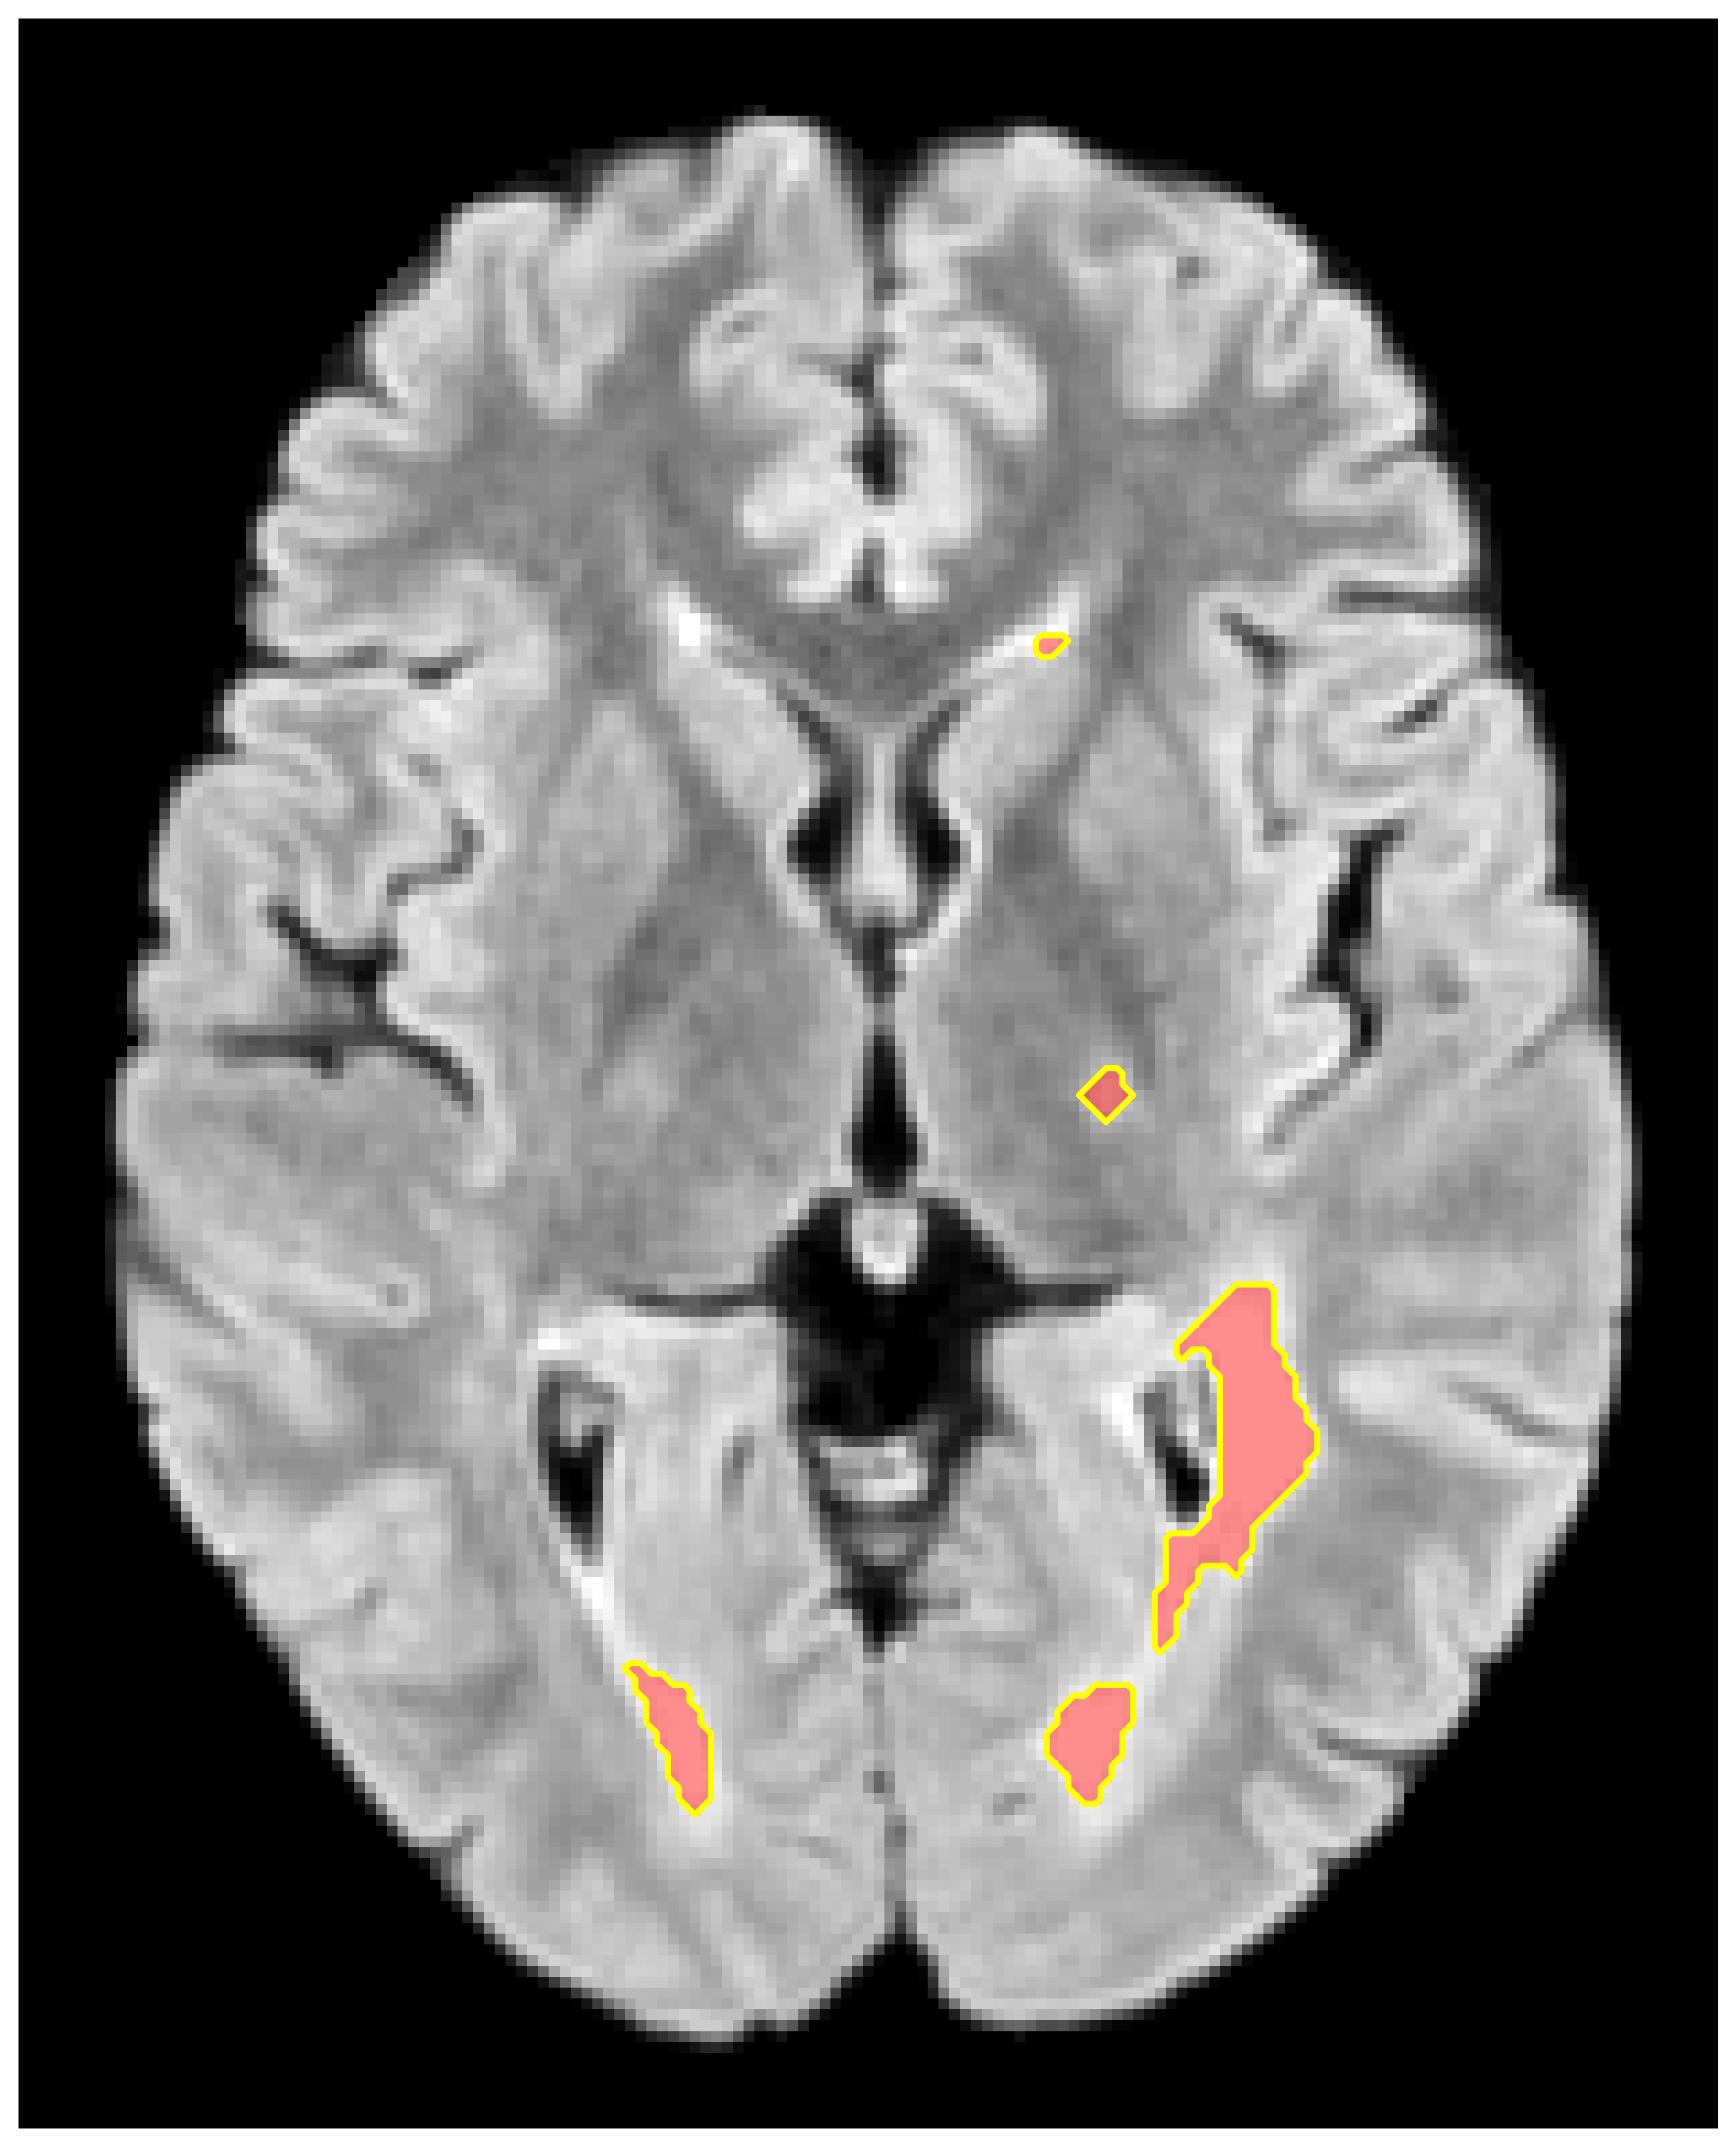
\includegraphics[width=\linewidth]{figures/flair_mask_overlay_slide.png}

  \end{columns}

\end{frame}

\begin{frame}{Problem}
\begin{columns}[T,totalwidth=\textwidth]

\column{0.6\textwidth}
\begin{itemize}
  \item Small lesions = \textbf{very few voxels} → extreme imbalance
  \item Loss dominated by \textbf{background / large lesions}
  \item \textbf{Small lesions → weak gradients → easily missed}
\end{itemize}

\vspace{0.2cm}
\begin{block}{Core challenge}
Ensure \textbf{each lesion contributes} to the optimization, not only large regions.
\end{block}

\column{0.38\textwidth}
\centering
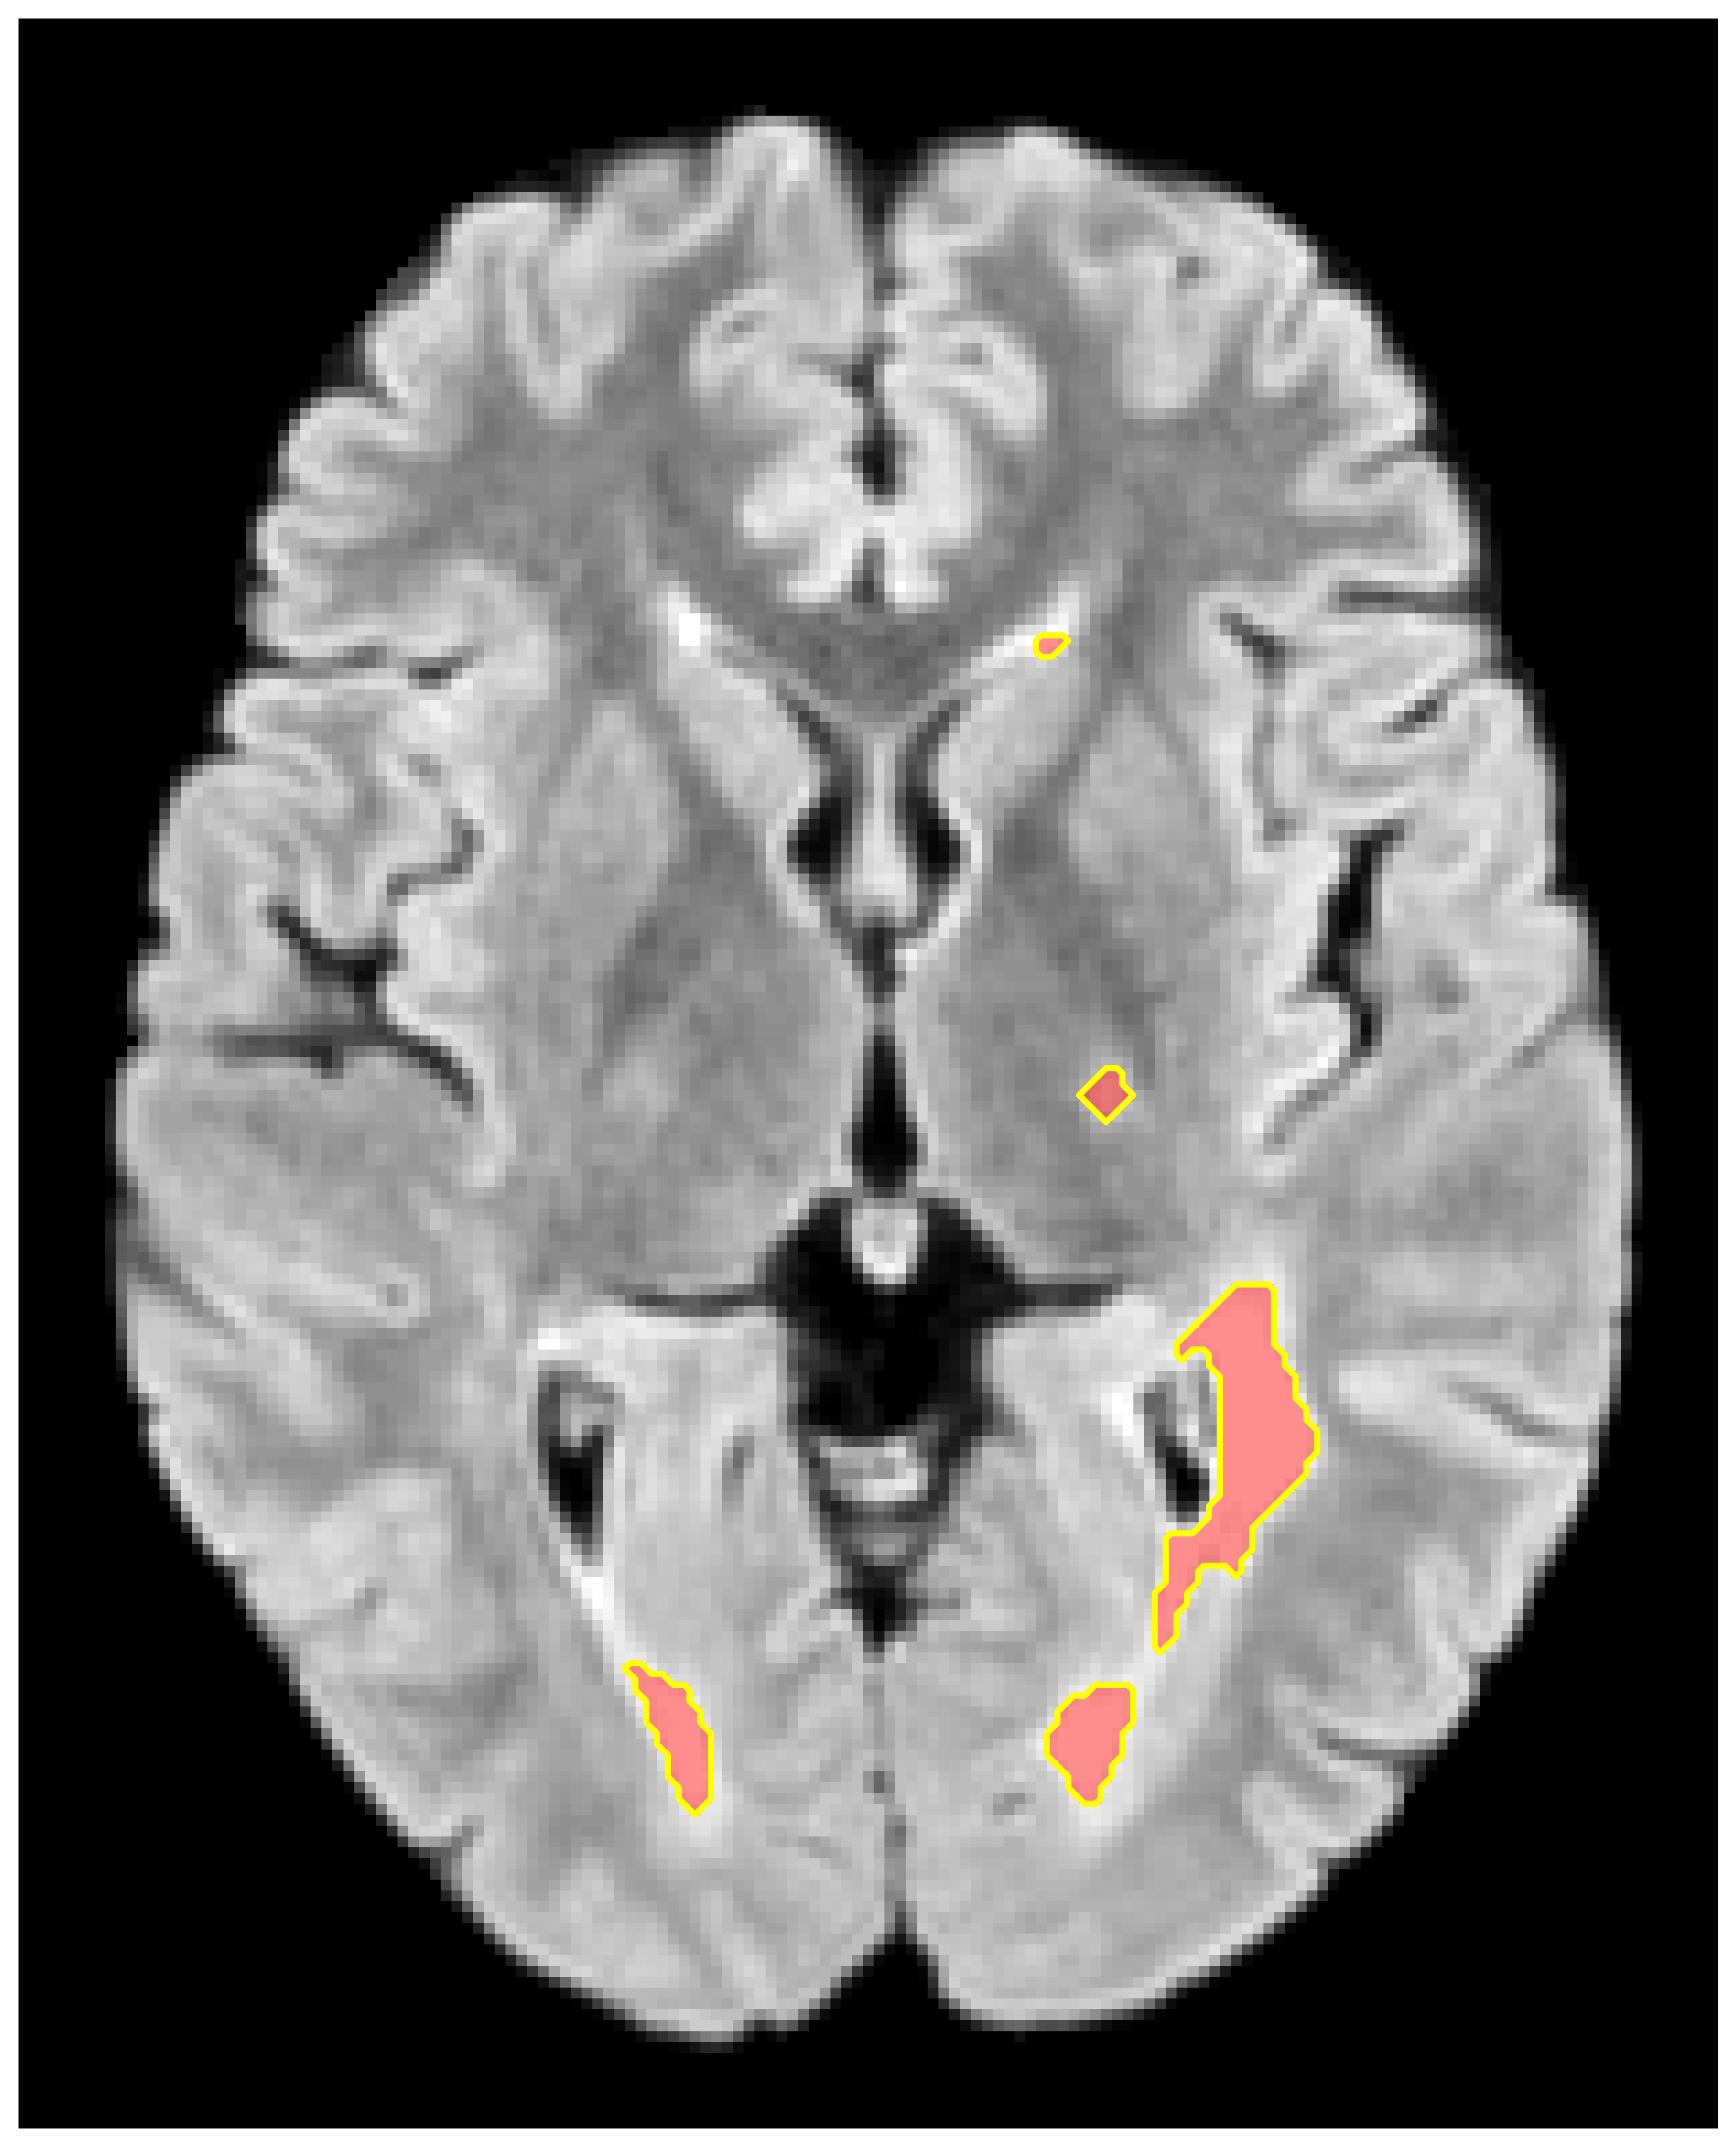
\includegraphics[width=0.9\linewidth]{figures/flair_mask_overlay_slide.png}

\vspace{0.15cm}

{\scriptsize
\begin{itemize}
  \item Overlap-based loss favors dense regions
  \item Voxel frequency ≠ lesion importance
\end{itemize}
}

\end{columns}
\end{frame}

\begin{frame}{Problem}
\begin{columns}[T,totalwidth=\textwidth]

\column{0.6\textwidth}
\begin{itemize}
  \item Small lesions = \textbf{very few voxels} → extreme imbalance
  \item Loss dominated by \textbf{background / large lesions}
  \item \textbf{Small lesions → weak gradients → easily missed}
\end{itemize}

\vspace{0.2cm}
\begin{block}{Core challenge}
Ensure \textbf{each lesion contributes} to the optimization, not only large regions.
\end{block}

\column{0.38\textwidth}
\centering
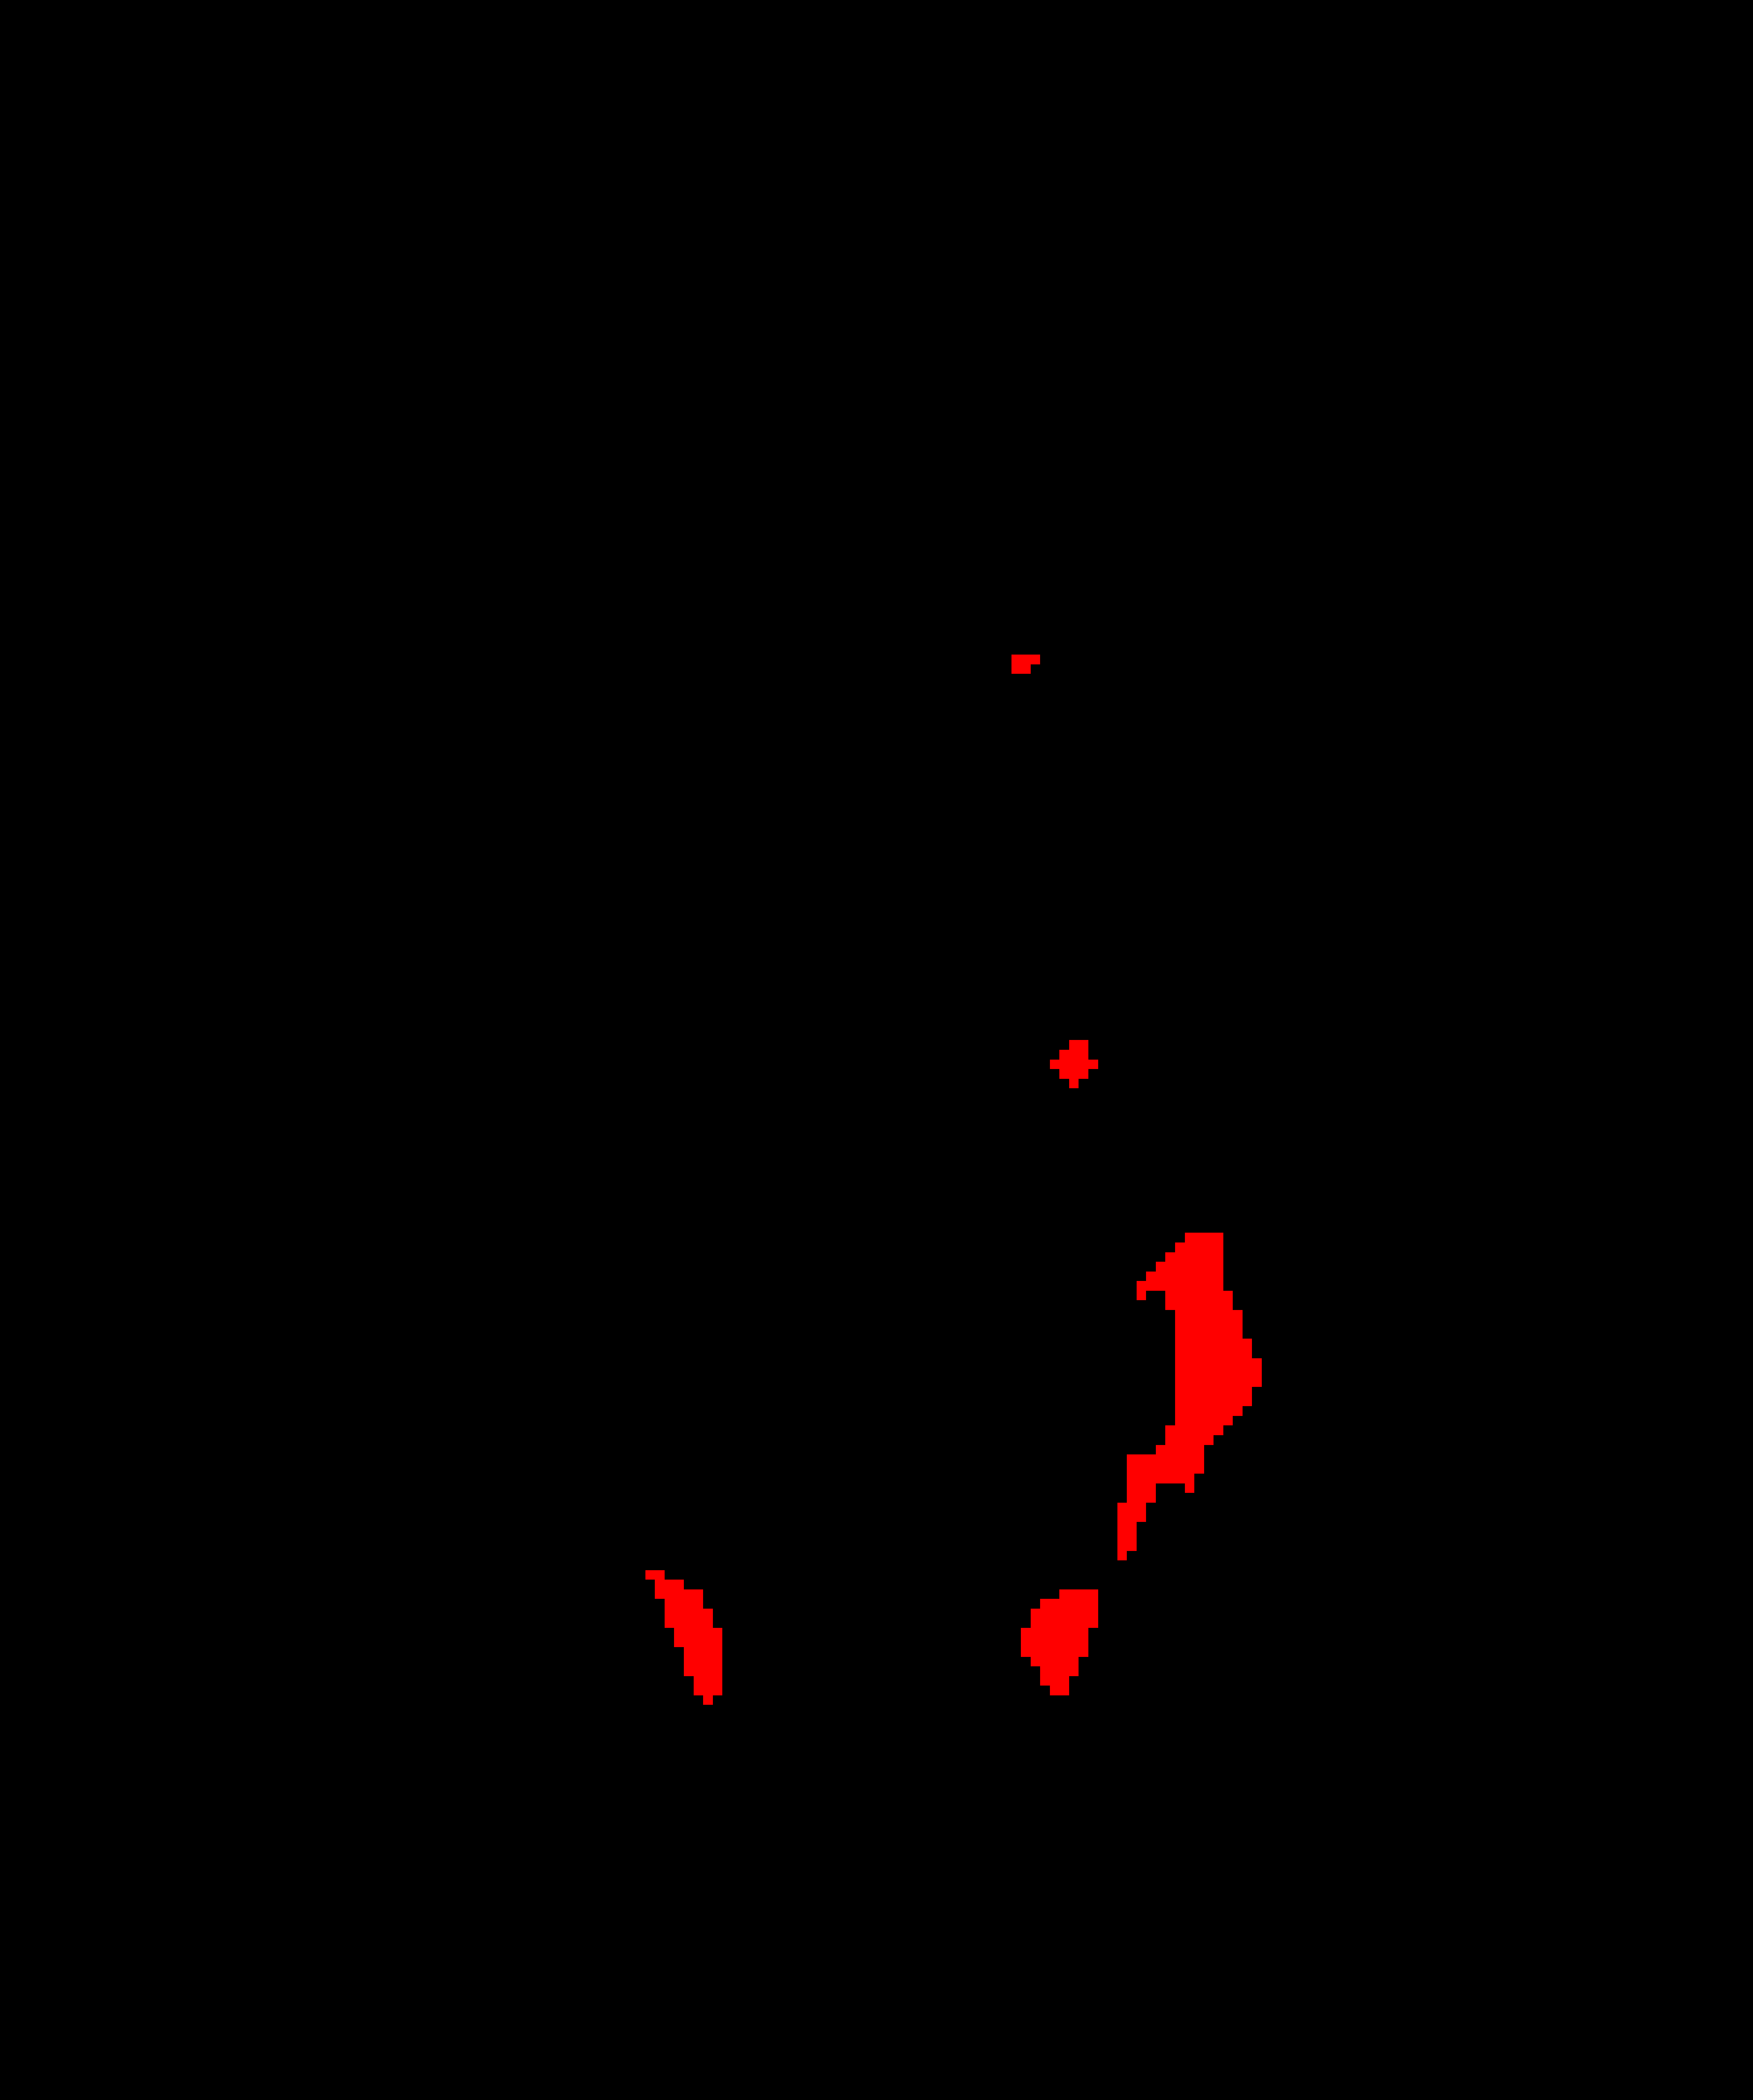
\includegraphics[width=0.9\linewidth]{figures/mask_only_red_fullsize.png}

\vspace{0.15cm}

{\scriptsize
\begin{itemize}
  \item Overlap-based loss favors dense regions
  \item Voxel frequency ≠ lesion importance
\end{itemize}
}

\end{columns}
\end{frame}

\begin{frame}{Hypothesis}

\begin{columns}[T,totalwidth=\textwidth]

%---------------- Left ----------------%
\column{0.55\textwidth}

\begin{block}{Key observation}
\small
\begin{itemize}
  \item Small lesions are \textbf{sparse} and occupy very few voxels
  \item Voxel-wise losses allocate signal \textbf{proportional to size}
  \item $\Rightarrow$ Small lesions receive \textbf{weak gradients}
\end{itemize}
\end{block}

\vspace{0.2cm}

\begin{block}{Limitation of standard supervision}
\small
\begin{itemize}
  \item Optimization dominated by \textbf{background and large lesions}
  \item Errors on small lesions are \textbf{under-penalized}
  \item High Dice $\neq$ reliable \textbf{lesion detection}
\end{itemize}
\end{block}

\vspace{0.2cm}

\begin{block}{Design principle}
\small
\centering
Reallocate the \textbf{optimization signal} so that \\
\textbf{sparse lesions have sufficient influence}
\end{block}

%---------------- Right ----------------%
\column{0.43\textwidth}

\begin{block}{Hypothesis}
\small
If supervision is restructured by:
\begin{itemize}
  \item \textbf{Structure-level balancing}
  \item \textbf{Lesion-level detection constraint}
\end{itemize}
then the model learns a better representation of \textbf{sparse lesions}
\end{block}

\vspace{0.3cm}

\begin{alertblock}{Expected effect}
\small
\centering
Higher \textbf{small-lesion recall} \\
Lower \textbf{false negatives} \\
Preserved \textbf{global performance}
\end{alertblock}

\end{columns}

\end{frame}


\begin{frame}{Proposed Objective Function}

\begin{columns}[T,totalwidth=\textwidth]

%---------------- Left: CAT ----------------%
\column{0.48\textwidth}
\begin{block}{\centering CAT (Component-Adaptive Tversky term)}
\small
\begin{align*}
\mathrm{I}_{\mathrm{CAT}} 
&= \frac{\mathrm{TP}_w}
{\mathrm{TP}_w + \alpha \mathrm{FP}_w + \beta \mathrm{FN}_w} \\[0.2cm]
\mathrm{TP}_w &= \sum_{i} w_i \, p_i g_i
\end{align*}

\vspace{-0.2cm}
\scriptsize
\begin{itemize}
  \item $w_i \propto (|C_k| + \epsilon)^{-1}$
  \item \textbf{Small lesions $\rightarrow$ higher weight}
  \item Equalizes contribution across components
\end{itemize}
\end{block}


%---------------- Right: MIL ----------------%
\column{0.48\textwidth}
\begin{block}{\centering MIL (Multiple Instance Learning term)}
\small
\begin{align*}
s_k &= \max_{i \in C_k} p_i \\[0.2cm]
\mathcal{L}_{\mathrm{MIL}} 
&= \frac{1}{K}\sum_{k=1}^{K} -\log(s_k + \epsilon)
\end{align*}

\vspace{-0.2cm}
\scriptsize
\begin{itemize}
  \item Each lesion = one instance $C_k$
  \item Requires \textbf{at least one confident voxel}
  \item Penalizes \textbf{missed lesions}
\end{itemize}
\end{block}

\end{columns}

\vspace{0.4cm}

%---------------- Bottom: Combined ----------------%
\begin{block}{\centering Final Objective}
\small
\[
\mathcal{L}_{\mathrm{CATMIL}} =
\mathcal{L}_{\mathrm{Dice}} + \mathcal{L}_{\mathrm{CE}}
+ \lambda_{\mathrm{CAT}} \mathcal{L}_{\mathrm{CAT}}
+ \lambda_{\mathrm{MIL}} \mathcal{L}_{\mathrm{MIL}}
\]
\end{block}

\vspace{-0.2cm}
\centering
{\scriptsize Combines voxel-, structure-, and lesion-level supervision}

\end{frame}

\begin{frame}{Experiment setup}
\begin{columns}[T,totalwidth=\textwidth]
\column{0.56\textwidth}
\begin{block}{Data and protocol}
\small
\begin{itemize}
  \item \textbf{Dataset:} MSLesSeg longitudinal brain MRI
  \item 75 subjects total; 53 with manual lesion annotations used for model development
  \item Modalities: \textbf{T1-w, T2-w, FLAIR}
  \item Preprocessed by organizers: skull stripping, co-registration to MNI152, resampled to \textbf{1 mm isotropic}
  \item Patient-level split to prevent longitudinal leakage
  \item \textbf{5-fold cross-validation} within nnU-Net; held-out 10\% independent test patients
\end{itemize}
\end{block}

\column{0.40\textwidth}
\begin{block}{Models compared}
\small
\begin{itemize}
  \item nnUNet-DiceCE
  \item nnUNet-Tversky
  \item nnUNet-FocalTversky
  \item \textbf{nnUNet-CATMIL} (proposed)
\end{itemize}
\end{block}

\begin{block}{Training details}
\small
\begin{itemize}
  \item nnUNet v2.1.1
  \item NVIDIA Quadro RTX 8000
  \item 150 epochs, batch size 2
  \item Adam, initial LR = 0.01
  \item Metrics: Dice, HD95, lesion F1, small-lesion recall, FN count, FN volume fraction, FP volume
\end{itemize}
\end{block}
\end{columns}
\end{frame}

\begin{frame}{Quantitative results}
\begin{columns}[T,totalwidth=\textwidth]
\column{0.39\textwidth}
\begin{block}{Main findings}
\small
\begin{itemize}
  \item \best{Best Dice} and \best{best HD95}
  \item \improve{Small-lesion recall: 0.8730}
  \item \improve{FN count: 2.57} vs 4.95 for DiceCE
  \item \improve{Lowest FP volume: 1537 mm$^3$}
  \item Trade-off: \tradeoff{lower lesion F1} than DiceCE / FocalTversky
\end{itemize}
\end{block}

\vspace{0.15cm}
\begin{block}{Interpretation}
\small
CATMIL delivers the \textbf{best balance between sensitivity and error control}, especially for small lesions.
\end{block}

\column{0.59\textwidth}
\scriptsize
\centering
\begin{tabular}{>{\raggedright\arraybackslash}p{2.6cm}cccc}
\toprule
\textbf{Metric} & \textbf{CATMIL} & \textbf{DiceCE} & \textbf{Tversky} & \textbf{FocalTv} \\
\midrule
Dice $\uparrow$ & \best{0.7834} & 0.7796 & 0.7706 & 0.7802 \\
HD95 (mm) $\downarrow$ & \best{7.9817} & 9.0372 & 10.2408 & 8.2060 \\
Small lesion recall $\uparrow$ & \best{0.8730} & 0.7956 & 0.8336 & 0.8313 \\
Lesion F1 $\uparrow$ & 0.7571 & 0.8433 & 0.8402 & \best{0.8455} \\
FN count $\downarrow$ & \best{2.5667} & 4.9500 & 3.7667 & 3.7000 \\
FN volume frac. $\downarrow$ & \best{0.0214} & 0.0341 & 0.0257 & 0.0250 \\
FP volume (mm$^3$) $\downarrow$ & \best{1537} & 1819 & 2621 & 2282 \\
\bottomrule
\end{tabular}
\vspace{0.15cm}

{\tiny Higher is better for Dice, lesion F1, and small-lesion recall; lower is better for HD95 and error metrics.}
\end{columns}
\end{frame}

\begin{frame}{Qualitative results: P47-T1}
\centering
\includegraphics[width=0.5\textwidth]{figures/P47_T1_fold1_slice94_segmentation_comparison.jpeg}

\vspace{0.3cm}

{\small 
\textbf{Clustered lesions with moderate contrast.}\\
CATMIL recovers additional small lesions and produces more coherent boundaries.
}

\vspace{0.2cm}
{\tiny Color code: green = correct, red = false negatives, yellow = false positives.}
\end{frame}


\begin{frame}{Qualitative results: P49-T2}
\centering
\includegraphics[width=0.5\textwidth]{figures/P49_T2_fold1_slice90_segmentation_comparison.jpeg}

\vspace{0.3cm}

{\small 
\textbf{Low-contrast, elongated lesions with blurred boundaries.}\\
CATMIL detects more difficult regions while limiting false alarms.
}

\vspace{0.2cm}
{\tiny Color code: green = correct, red = false negatives, yellow = false positives.}
\end{frame}


\begin{frame}{Qualitative results: P52-T2}
\centering
\includegraphics[width=0.5\textwidth]{figures/P52_T2_fold0_slice87_segmentation_comparison.jpeg}

\vspace{0.3cm}

{\small 
\textbf{Extreme sparse-lesion setting.}\\
CATMIL preserves main lesions while introducing a small isolated false positive.
}

\vspace{0.2cm}
{\tiny Color code: green = correct, red = false negatives, yellow = false positives.}
\end{frame}

% \begin{frame}{Qualitative results: three cases}
% \centering
% \begin{columns}[T,totalwidth=\textwidth]
% \column{0.32\textwidth}
% \includegraphics[width=\linewidth]{figures/P47_T1_fold1_slice94_segmentation_comparison.jpeg}
% \vspace{0.1cm}

% {\scriptsize \textbf{P47-T1}\\Clustered lesions with moderate contrast.\\CATMIL recovers additional small lesions and gives more coherent boundaries.}

% \column{0.32\textwidth}
% \includegraphics[width=\linewidth]{figures/P49_T2_fold1_slice90_segmentation_comparison.jpeg}
% \vspace{0.1cm}

% {\scriptsize \textbf{P49-T2}\\Low-contrast, elongated lesions with blurred boundaries.\\CATMIL detects more difficult regions while limiting false alarms.}

% \column{0.32\textwidth}
% \includegraphics[width=\linewidth]{figures/P52_T2_fold0_slice87_segmentation_comparison.jpeg}
% \vspace{0.1cm}

% {\scriptsize \textbf{P52-T2}\\Extreme sparse-lesion setting.\\CATMIL keeps main lesions localized, but may add a small isolated false positive.}
% \end{columns}

% \vspace{0.15cm}
% {\tiny Color code from the dissertation figures: green = correct lesion voxels, red = false negatives, yellow = false positives.}
% \end{frame}

\begin{frame}{Discussion}
\begin{columns}[T,totalwidth=\textwidth]
\column{0.49\textwidth}
\begin{block}{Takeaways}
\small
\begin{itemize}
  \item Small-lesion segmentation is fundamentally a \textbf{sparse representation learning} problem.
  \item Loss design can change model behavior without adding architectural complexity.
  \item CATMIL improves \textbf{sensitivity to subtle lesions} and reduces false negatives.
  \item Global segmentation quality remains stable while boundary accuracy improves.
\end{itemize}
\end{block}

\column{0.49\textwidth}
\begin{block}{Limitations and future work}
\small
\begin{itemize}
  \item \risk{Trade-off:} increased sensitivity lowers lesion-wise precision in some cases.
  \item Evaluated on a \textbf{single dataset}, disease, and architecture.
  \item Future work: multi-dataset validation, extension to other brain pathologies, and explicit control of the \textbf{detection--precision} trade-off.
\end{itemize}
\end{block}

\vspace{0.15cm}
\begin{block}{Bottom line}
\small Combining \textbf{structure-level balancing} and \textbf{lesion-level constraints} yields a more robust encoding of small, sparse pathological signals.
\end{block}
\end{columns}
\end{frame}

\begin{frame}{Next Plan}

\begin{columns}[T,totalwidth=\textwidth]

%---------------- Left ----------------%
\column{0.52\textwidth}

\begin{block}{1. Loss vs Architecture}
\small
\begin{itemize}
  \item Compare \textbf{different architectures}
  \item Keep loss functions consistent
  \item Isolate:
  \begin{itemize}
    \item representation effect
    \item vs objective design
  \end{itemize}
\end{itemize}
\end{block}

\vspace{0.25cm}

\begin{block}{2. Feature Analysis}
\small
\begin{itemize}
  \item Analyze embeddings of \textbf{FN lesions}
  \item Identify error source:
  \begin{itemize}
    \item weak representation
    \item vs decision boundary
  \end{itemize}
\end{itemize}
\end{block}


%---------------- Right ----------------%
\column{0.45\textwidth}

\begin{block}{3. Representation Design}
\small
\begin{itemize}
  \item Modify architecture \textbf{only if needed}
  \item Focus on:
  \begin{itemize}
    \item sparse signal encoding
    \item small lesion sensitivity
  \end{itemize}
\end{itemize}
\end{block}

\end{columns}

\end{frame}



%---------------- Thank You ----------------%
\begin{frame}[plain]
\centering
\vspace{1.5cm}

{\usebeamerfont{title}\color{navy}Thank you!\par}

\vspace{0.5cm}

\vfill

{\small Email: khue.luu@g.nsu.ru \\ Github: https://github.com/luumsk/SmallLesionMRI (in progress) \\ Paper: TBA}

\end{frame}

\end{document}
